\chapter[Gain and Lasing]{Stimulated Emission, Optical Gain and Lasing in Core-Shell Nanowires} \label{LT}

In this chapter, we review the history and operation principle of semiconductor
lasers, then through the derivation of the gain spectrum for different
dimensionality, the threshold carrier density and the quantum efficiency are
calculated, showing that lower dimensional structures are capable to generate
more output power due to the extremely enhanced optical transition rates. In
addition, a nanowire transient response model under ultrafast pulse excitation
is discussed, revealed the large carriers and optical power generated when
the excitation power above the threshold condition.

\section{Background of Semiconductor Lasers} \label{SLhistory} 

Semiconductor laser is an essential component for building optical
communication systems, while intensive research results and achievements are
published in this field. In 1917, Einstein predicted the existence of
spontaneous and stimulated emission as depicted in Fog.~\ref{Threelevel} by
which an atom can emit radiation~\cite{einstein1917quantum}. After the proposal
of p-n junction semiconductor lasers in 1961~\cite{basov1961generation}, the
first semiconductor lasers were fabricated in 1962 using
homojunctions~\cite{hall1962coherent}. These lasers have high threshold current
density ($19000/A/{cm}^2$) and operated at very low temperature, thus, not
efficient enough due to high optical and electrical losses. The concept of
heterojuntion or double heterojunction semiconductor lasers were realized in
the late 1960s by Alferov and others with a lower threshold current density
($1600 A/{cm}^2$) operating at room temperature~\cite{alferov1970alas}. These
double-heterostructure diode lasers provide both carrier and optical
confinements, which improve the efficiency for stimulated emission. The concept
of quantum well structures for semiconductor lasers was proposed and realized
experimentally in the late 1970s. In these lasers the active region, in which
electrons and holes recombine to give off light, is less than
$100\text{\normalfont\AA}$ wide. Such small transverse dimensions are obtained
using molecular beam epitaxy and employ most often a GaAs active region
sandwiched between higher energy band gap materials layers, such as AlGaAs. The
threshold current density was reduced to less than 500 $A/{cm}^2$, which
improved the laser performance significantly.

\section{Operation Principle of Semiconductor Lasers} \label{SLoperation}

The semiconductor laser (or laser diode) in its simplest form is a p-n junction
of semiconductor material arranged in a cavity, as shown
in~\ref{LaserStructure}. Two metal contacts connected to the p-type or n-type
semiconductor materials separately with a junction active region in between. On
the optically flat and parallel side faces, there are two mirror like
reflectors to confine and forming the feedback of light, in order to produce
coherent radiation at one side of the device.  The type and configuration of
the material used determine the optical characteristics of the laser diode
emission. Like others in various oscillators or wave sources, the fundamental
elements in the semiconductor lasers are the following three elements:

\begin{figure}
  \caption[Basic structure of a junction laser in the form of a Fabry-Perot cavity, showing the active region and the coherent radiation output.]{Basic structure of a junction laser in the form of a Fabry-Perot cavity, showing the active region and the coherent radiation output. Figure adapted from the reference~\cite{sze2006physics}.}
  \centering
  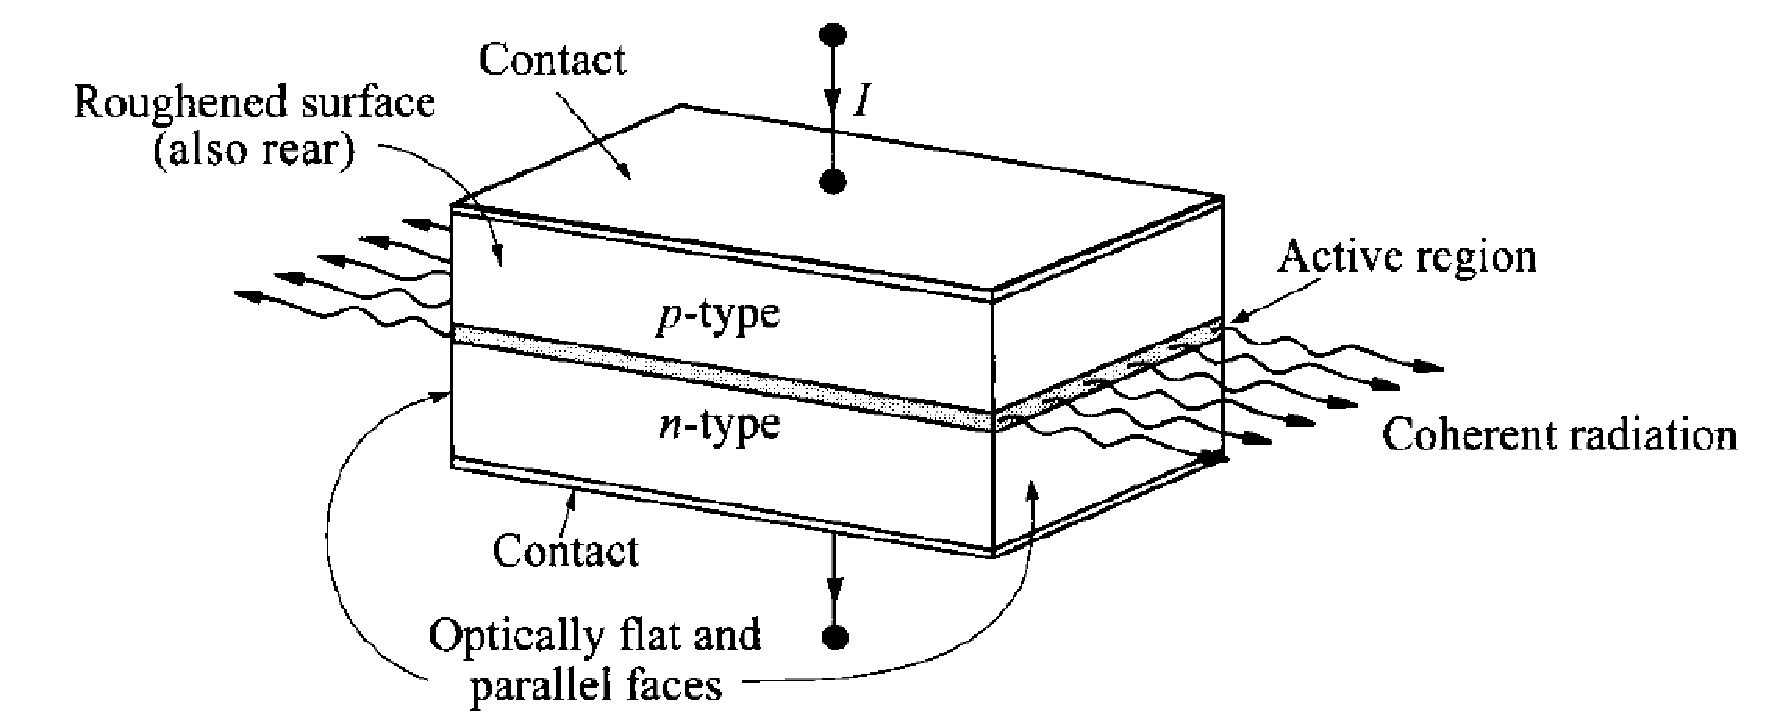
\includegraphics[width=\textwidth]{pictures/LT/LaserStructure}
  \label{LaserStructure}
\end{figure}

\begin{itemize}
  \item \textbf{Population Inversion} In order to provide net optical gain and achieve non-equilibrium condition, electrons must be excited to a highly excited level as depicted in a three level laser in Fig.~\ref{Threelevel}. The excited electrons will recombine radiationless with holes and release their energy to the upper level, where the population of electrons will be greater than the population in ground state, and achieving population inversion with optical amplification.
  \item \textbf{External Pumping and p-n Junction} Either electrical injection or optical pumping can provide the source of input energy and optical radiation obtained by injecting minority carriers into the vicinity of a semiconductor p-n junction where radiative transitions take place.
  \item \textbf{Reflectors of Cavity} The structural requirement for a laser is an optical resonator in the direction of the light output. The optical resonator mainly serves to trap the light and build up the intensity inside. Based on the types of reflector, the most common semiconductor lasers are including Fabry-Perot(FP) lasers~\cite{Duan:2003en} or distributed feedback (DFB)~\cite{wang2015room}/distributed Bragg reflector (DBR)~\cite{chen2006nanowire} lasers.
\end{itemize}

\begin{figure}
  \caption{(left) Optical Process (absorption and emission) in a two level system. (right) Lasing mechanism with stimulated emission and population inversion in a three-levels system.}
  \centering
  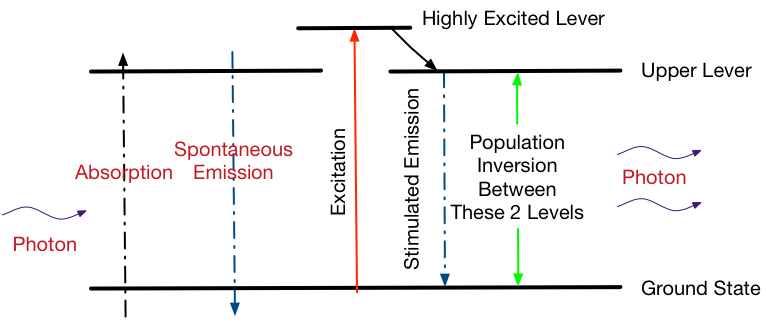
\includegraphics[width=\textwidth]{pictures/LT/Threelevel}
  \label{Threelevel}
\end{figure}

\section{Lasing Characteristics}
\subsection{Absorption of Light}

The light and matter interaction includes absorption, spontaneous emission and
stimulated emission. We first quantify the enhancement of absorption of light caused by reduced dimensionality by introducing
the absorption coefficient. This is the absorption rate without considering the
occupation factors. As derived in Chapter~\ref{RM}, the absorption
coefficient for 3D can be expressed as:

\begin{eqnarray}
    \alpha_{3D}(\hbar\omega)= & C_0{|\hat{e}\cdot\bf{p}_{cv}|^2}(f_v-f_c) \frac{1}{2\pi^2}(\frac{2m_r^\ast}{\hbar^2})^{3/_2}(\hbar\omega-E_g)^{1/_2}, \nonumber \\
    & C_0=\frac{\pi{e^2}}{n_r\epsilon_0{c}{m_0^2}\omega},
    \label{eq:abs_3D}
\end{eqnarray}

and for 2D and 1D case, we have:
\begin{eqnarray}
\begin{aligned}
& \alpha_{2D}(\hbar\omega)=C_0{|\hat{e}\cdot\bf{p}_{cv}|^2}\frac{m_r^\ast}{\pi\hbar^2{L_z}},
\\
& \alpha_{1D}(\hbar\omega)=C_0{|\hat{e}\cdot\bf{p}_{cv}|^2}\frac{{(m_r^\ast)}^{3/_2}}{\pi\hbar{m_e^\ast}{L_x}{L_y}}\frac{1}{\sqrt{(\hbar\omega-E_g)}},
    \label{eq:abs_2D}
\end{aligned}
\end{eqnarray}

The split plots of absorption coefficient for 3D, 2D and 1D are shown in
Fig.~\ref{absrate_split}. Note the unique shapes of joint optical density of
states (JODS), i.e., from continuous JODS for 3D to step-like JODS for 2D, and
discrete form for 1D, as explicitly shown in the last terms of
Eqs.~(\ref{eq:abs_3D} and~\ref{eq:abs_2D}). The parameters used for rate
equations calculation are presented in table~\ref{tab:rate_eq}.
\setlength{\tabcolsep}{4pt}

\begin{deluxetable}{lll}
\tabletypesize{\footnotesize}
\tablewidth{0pt}

\tablecaption{Parameters and constants used for rate equation calculations. \label{tab:rate_eq}}
\tablehead{\colhead{Parameters} & \colhead{Symbol} & \colhead{Values and Units}}
\startdata
Reduced Planck's constant               &   {\em $\hbar$}        &  $1.05\times10^{-34}~J\cdot{s}$\\
Speed of light                          &   {\em $c$}          &  $3\times10^10$~$m/s$\\
Elementary charge                       &   {\em e}            &  $1.6\times10^{-19}~C$\\
Energy Bandgap for GaAs at 300k         &   {\em $E_{g}$}      &  $1.424~eV$ \\
Permeability of vacuum                  &   {\em $\mu_0$}      &  $4\pi\times10^{-7}~H/m$   \\
Permittivity of vacuum                  &   {\em $\varepsilon_0$}      &  $8.854\times10^{-12}~F/m$   \\
Electron rest mass                      &   {\em $m_{0}$}      &  $9.109\times10^{-31}~kg$ \\
Electron effective mass                 &   {\em $m_{e}$}      &  $0.067m_0$ \\
Hole effective mass for GaAs 3D         &   {\em $m_{h3D}$}    &  $0.47m_0$ \\
Hole effective mass for GaAs 2D         &   {\em $m_{h2D}$}    &  $0.118m_0$ \\
Hole effective mass for GaAs 1D         &   {\em $m_{h1D}$}    &  $0.027m_0$ \\
Thermal voltage at 300k                 &   {\em $V_{t}$}      &  $0.02585~eV$ \\
Energy Parameter for GaAs               &   {\em $E_{p}$}      &  $25.7~eV$ \\
\enddata
\tablecomments{The rest of the parameters that are not listed here have its conventional meaning and values.}
\end{deluxetable}

\begin{figure}
  \caption{Absorption Coefficient versus Photon Energy for 1D 2D and 3D with split plot.}
  \centering
  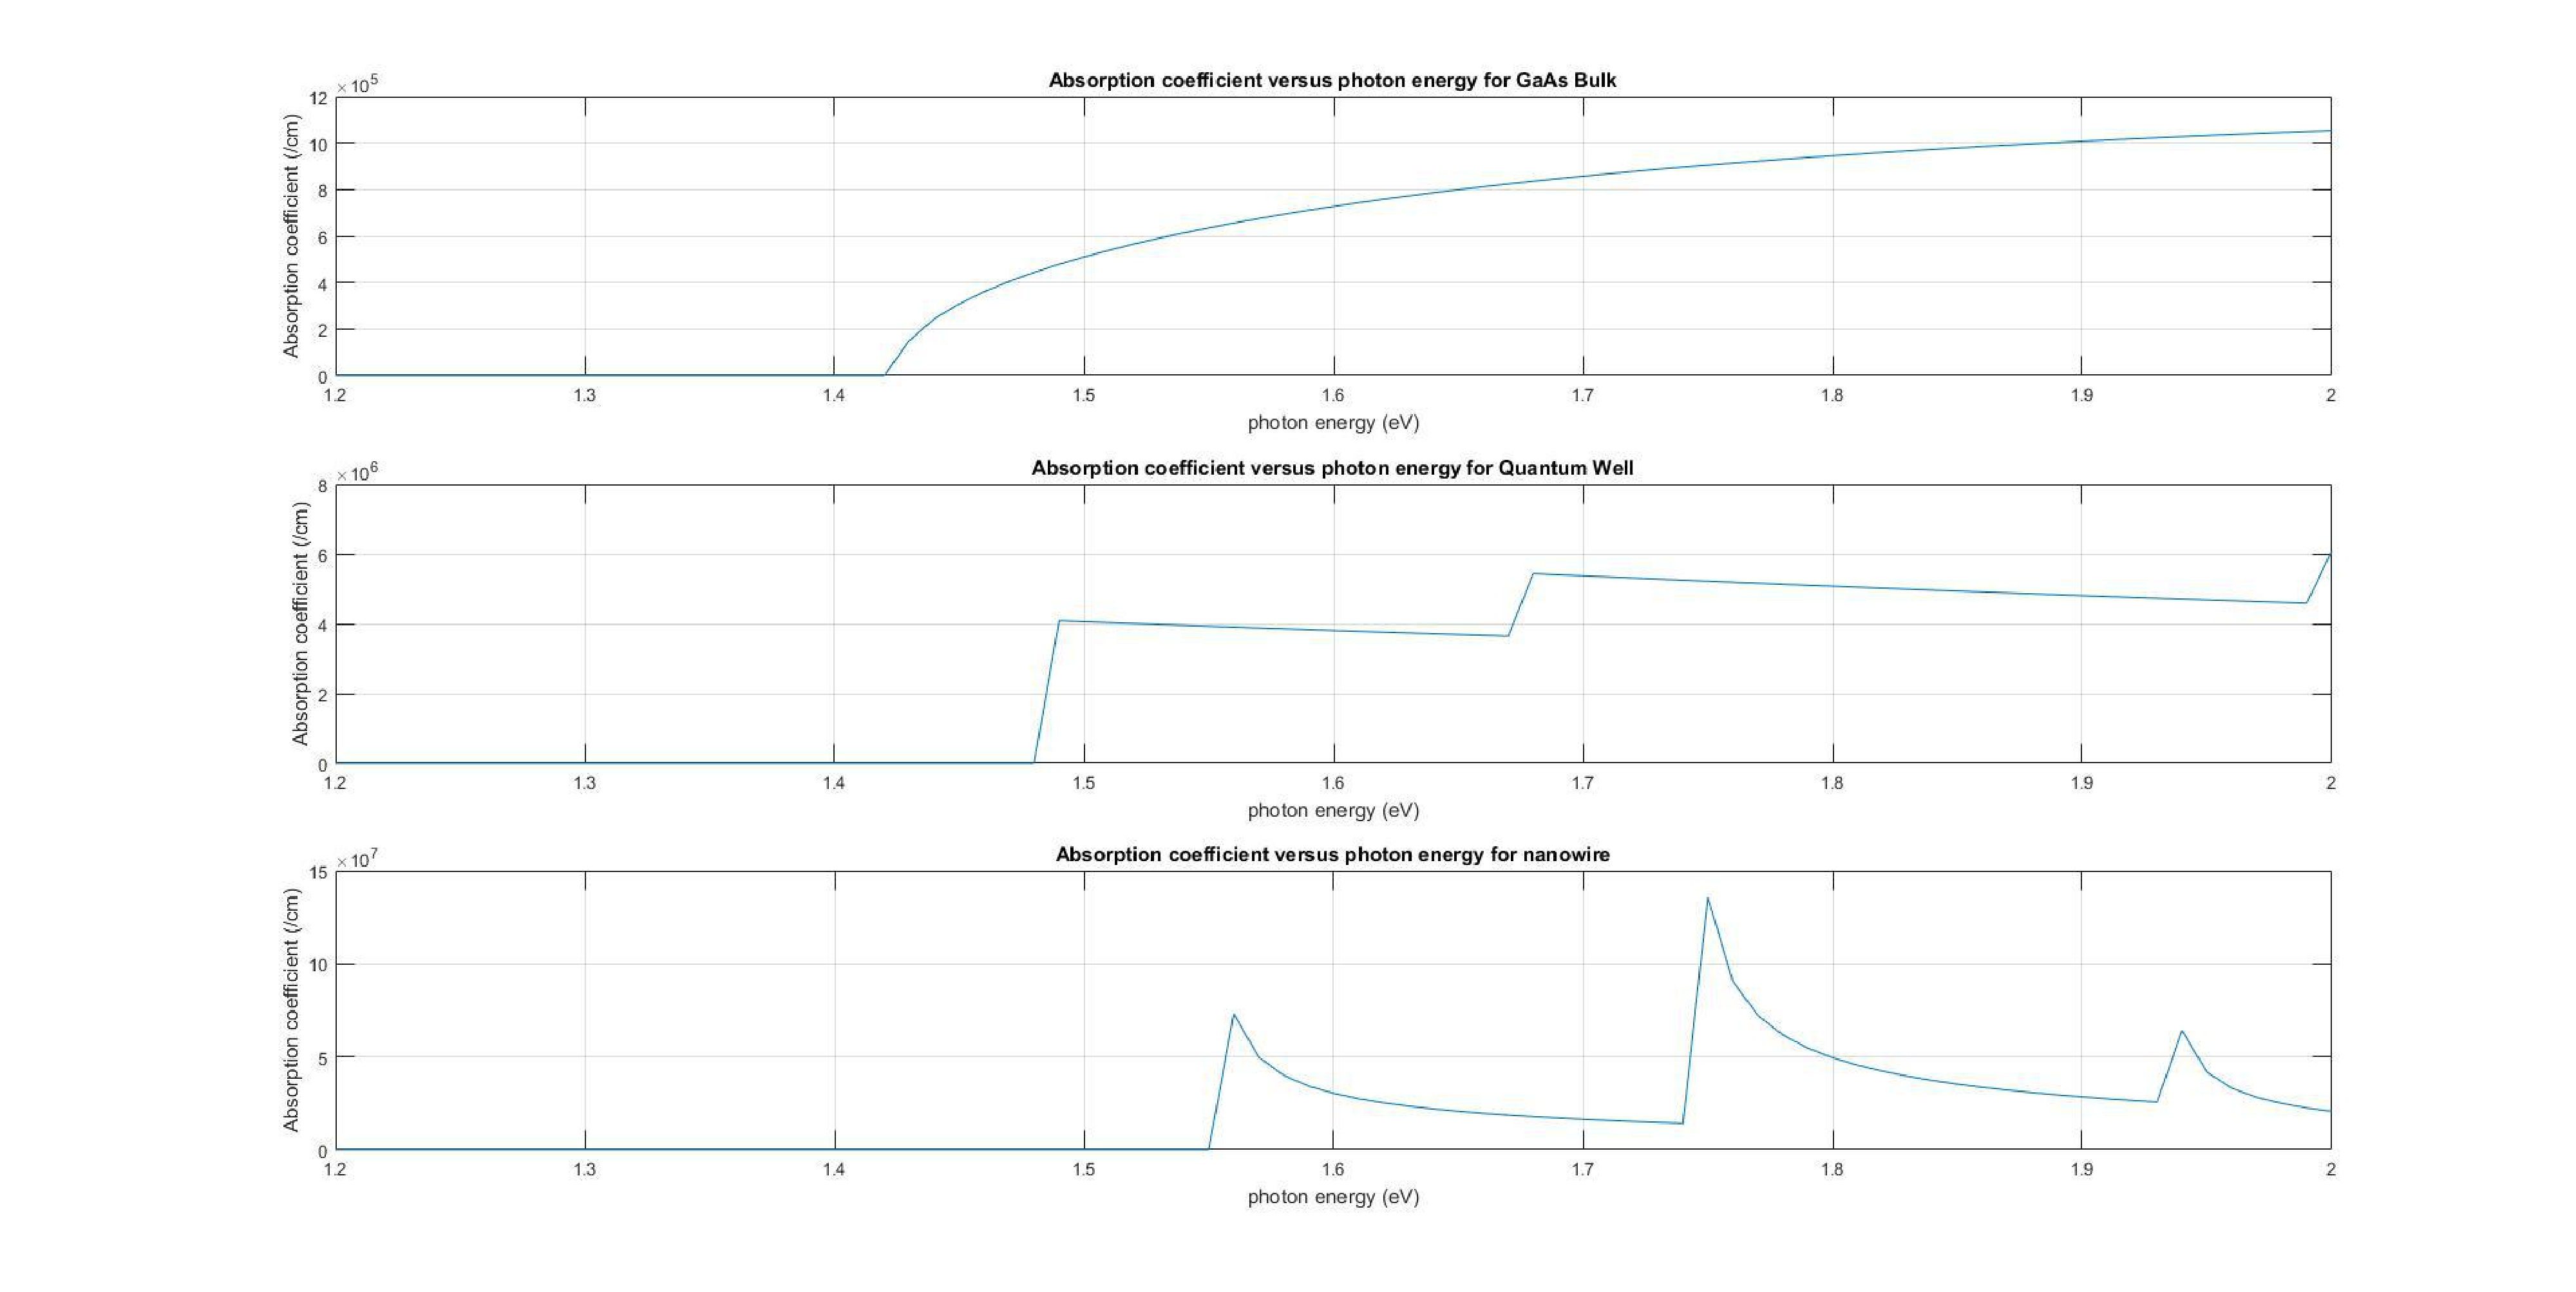
\includegraphics[width=\textwidth]{pictures/LT/absrate_split}
  \label{absrate_split}
\end{figure}

Then the overlay plot with multiple y axis as in Fig.~\ref{absrate_overlay}
with the different scales indicating the integrated absorption rates for 1D is
35 times larger than 3D. The maximum absorption coefficient is $1.0\times10^{6}
(cm^{-1})$ for 3D, $6.1\times10^{6} (cm^{-1})$ for 2D and $1.4\times10^{8}
(cm^{-1})$ for 1D.

\begin{figure}
  \caption{Absorption Coefficient versus Photon Energy for 1D, 2D and 3D with multiple y axis.}
  \centering
  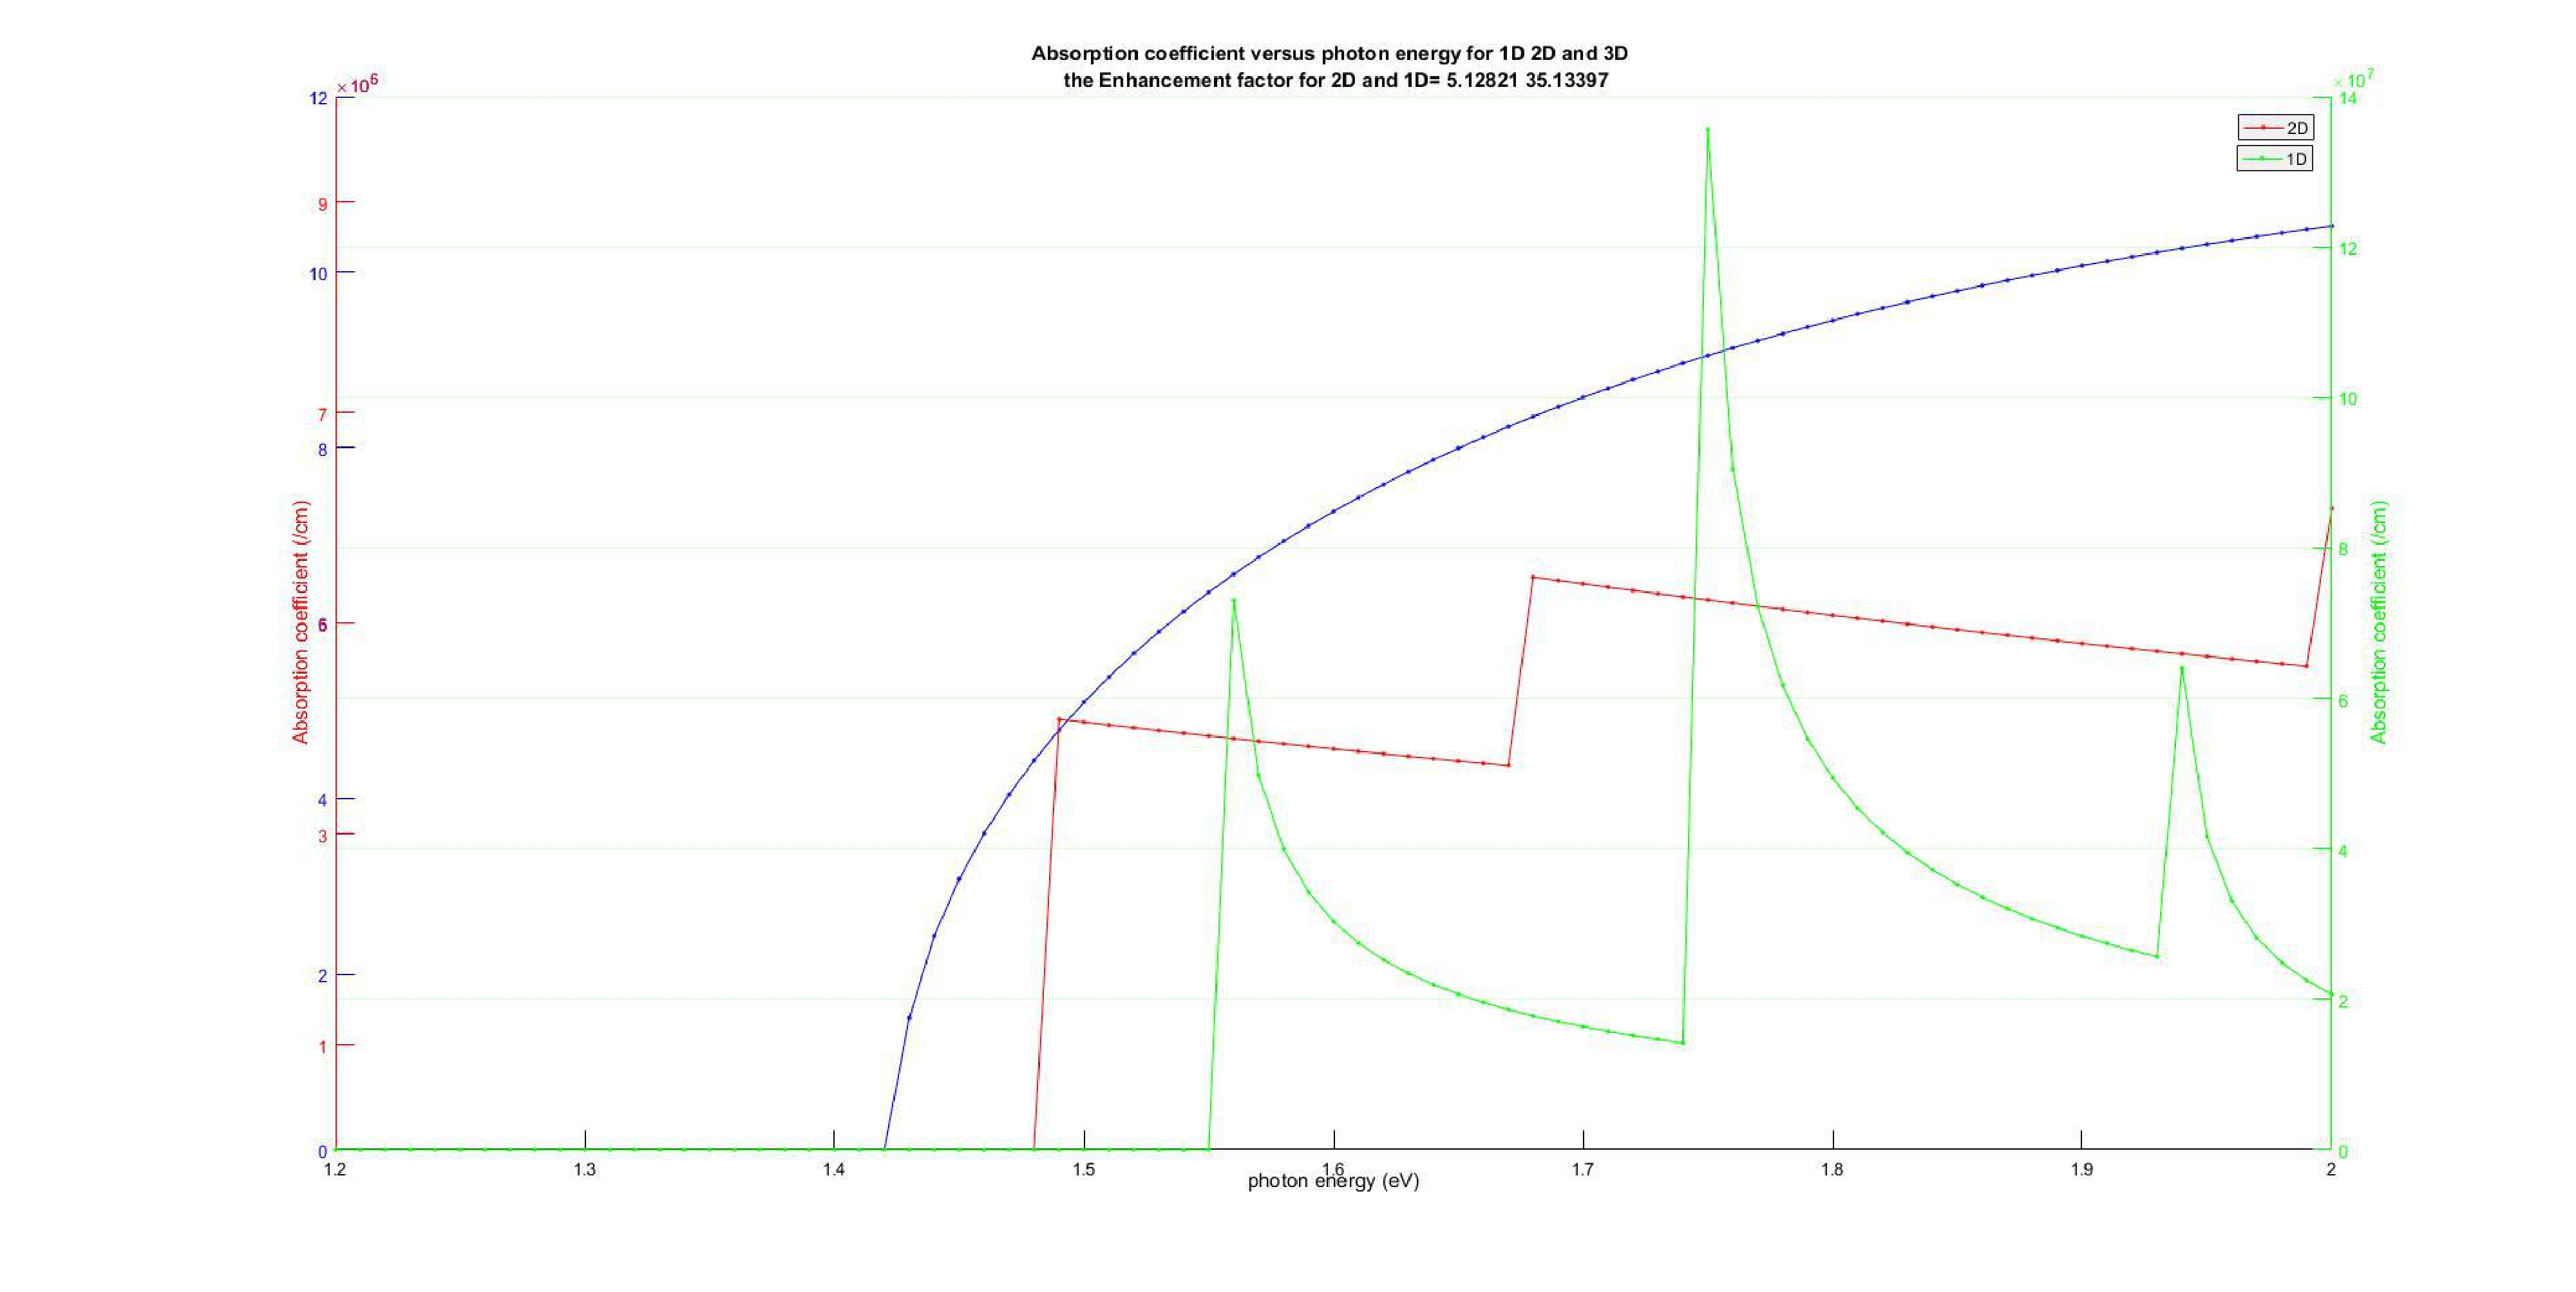
\includegraphics[width=\textwidth]{pictures/LT/absrate_overlay}
  \label{absrate_overlay}
\end{figure}

\subsection{Optical Gain}

The net stimulated emission rate is given by
$r_{\mathrm{sti}}^{\mathrm{net}}(\hbar\omega)=r_{\mathrm{sti}}(\hbar\omega)-\alpha_{\mathrm{abs}}(\hbar\omega)$,
and the optical gain is equal to the net stimulated emission rate divided by
the photon flux as
$g(\hbar\omega)=r_{\mathrm{sti}}^{\mathrm{net}}(\hbar\omega)/{(c{n_\varepsilon}u_\varepsilon/n_r)}$,
where $n_\varepsilon$ is the photon mode density. Thus, an expression for the
gain spectra $g(\hbar\omega)$ can be derived for 3D, 2D and
1D~\cite{coldren2012diode} with consideration also of occupation factor by
calculating the Fermi levels:

\begin{eqnarray}
\begin{aligned}
& g_{3D}(\hbar\omega)=\frac{\sqrt{2}e^2{m_r^\ast}^{3/2}{p_{cv}^2}}{3{\pi}n_r\epsilon_0{m_0}^2c{\hbar^3}\omega}{\sqrt{(\hbar\omega-E_g)}}(f_c-f_v),
\\
& g_{2D}(\hbar\omega)=\frac{e^2{m_r^\ast}{p_{cv}^2}}{3{n_r}\epsilon_0{m_0}^2c{\hbar^2}L_z\omega}(f_c-f_v),
\\
& g_{1D}(\hbar\omega)=\frac{e^2{m_r^\ast}^{3/2}{p_{cv}^2}}{3{n_r}\epsilon_0{m_0}^2c\hbar\omega{L_x}{L_y}}\frac{1}{\sqrt{(\hbar\omega-E_g)}}(f_c-f_v).
\end{aligned}
\label{eq:gainspectrum}
\end{eqnarray}

With decreasing dimensionality of the active region of an injection laser, the
joint optical density of states and gain spectra become narrower, which leads
to a decrease in the number of states to be filled to make the active region
transparent (zero population inversion and zero gain) and to achieve lasing
(round trip gain equal to loss). Consequently, the transparency current (or
inversion current, i.e., the injection current at which the population
inversion is zero) and the threshold current (injection current at which the
gain is equal to the loss and lasing begins) decrease and their temperature
dependence becomes weaker~\cite{asryan2004theory}. The decrease in the
threshold current and increase in its temperature stability reflect one of the
main areas of development and improvement of injection lasers. Owing to the
continuous nature of the carrier spectrum within the allowed subbands, the use
of quantum wells (QWs) or quantum well wires (QWRs) as active medium for
optical transitions can quantitatively improve the parameters of devices based
on them compared with devices with a bulk active region.

Among the advantages of QWR lasers over the presently used QW lasers are their
narrower gain spectra, much lower threshold currents, and ultrahigh temperature
stability, as well as the wider possibilities for controlling their lasing
wavelength.

Now the gain spectrum respect to photon energy for (a) 3D, (b) 2D and (c) 1D
can be calculated in Figure~\ref{gainspectrum}. As expected, the gain spectrum
also follows the unique shapes of density of states. The inset of
Fig.~\ref{gainspectrum}(a) is the maximum gain versus electron carrier
concentration varing from $3\times10^{18} (cm^{-3})$ to
$3\times10^{19}(cm^{-3})$. Using parameters $N_{tr} = 2\times10^{18} cm^{-3}$,
$N_{s} = 4\times10^{18} cm^{-3}$, and $g_0 = 6.11\times10^{5} cm^{-1}$, we fit
the curve in inset of Fig.~\ref{gainspectrum}(a) to build a logarithmic gain
model of the form for 3D case:

\begin{equation}
  g(N) = g_0\ln\left(\frac{N+N_s}{N_{tr}+ N_s}\right)
\end{equation}
where $N_s$ is a shift to force the natural logarithm to be finite at $N = 0$
such that the gain equals the unpumped absorption due to the band-to-band
transitions, $N_{tr}$ is the transparency carrier density, and $g_0$ is the
empirical gain coefficient. $N_{tr}$ and $g_0$ will be different for different
dimensionality.

\begin{figure}
  \caption[Gain coefficient and spontaneouse emission rate versus photon energy
  for different dimensionality.]{Gain Coefficient versus Photon Energy for (a)
    3D (b) 2D and (c) 1D as a function of carrier concentration. The inset of
    (a) is the maximum gain versus injected/pumped electron carrier
    concentration varing from $3\times10^{18} (cm^{-3})$ to
    $3\times10^{19}(cm^{-3})$. (d) Spontaneous Emission Rate versus Photon
    Energy with respect to threshold carrier concentration for 3D(green),
    2D(red) and 1D(blue). Note the scales difference for different
  dimensionality cases.}
  \centering
  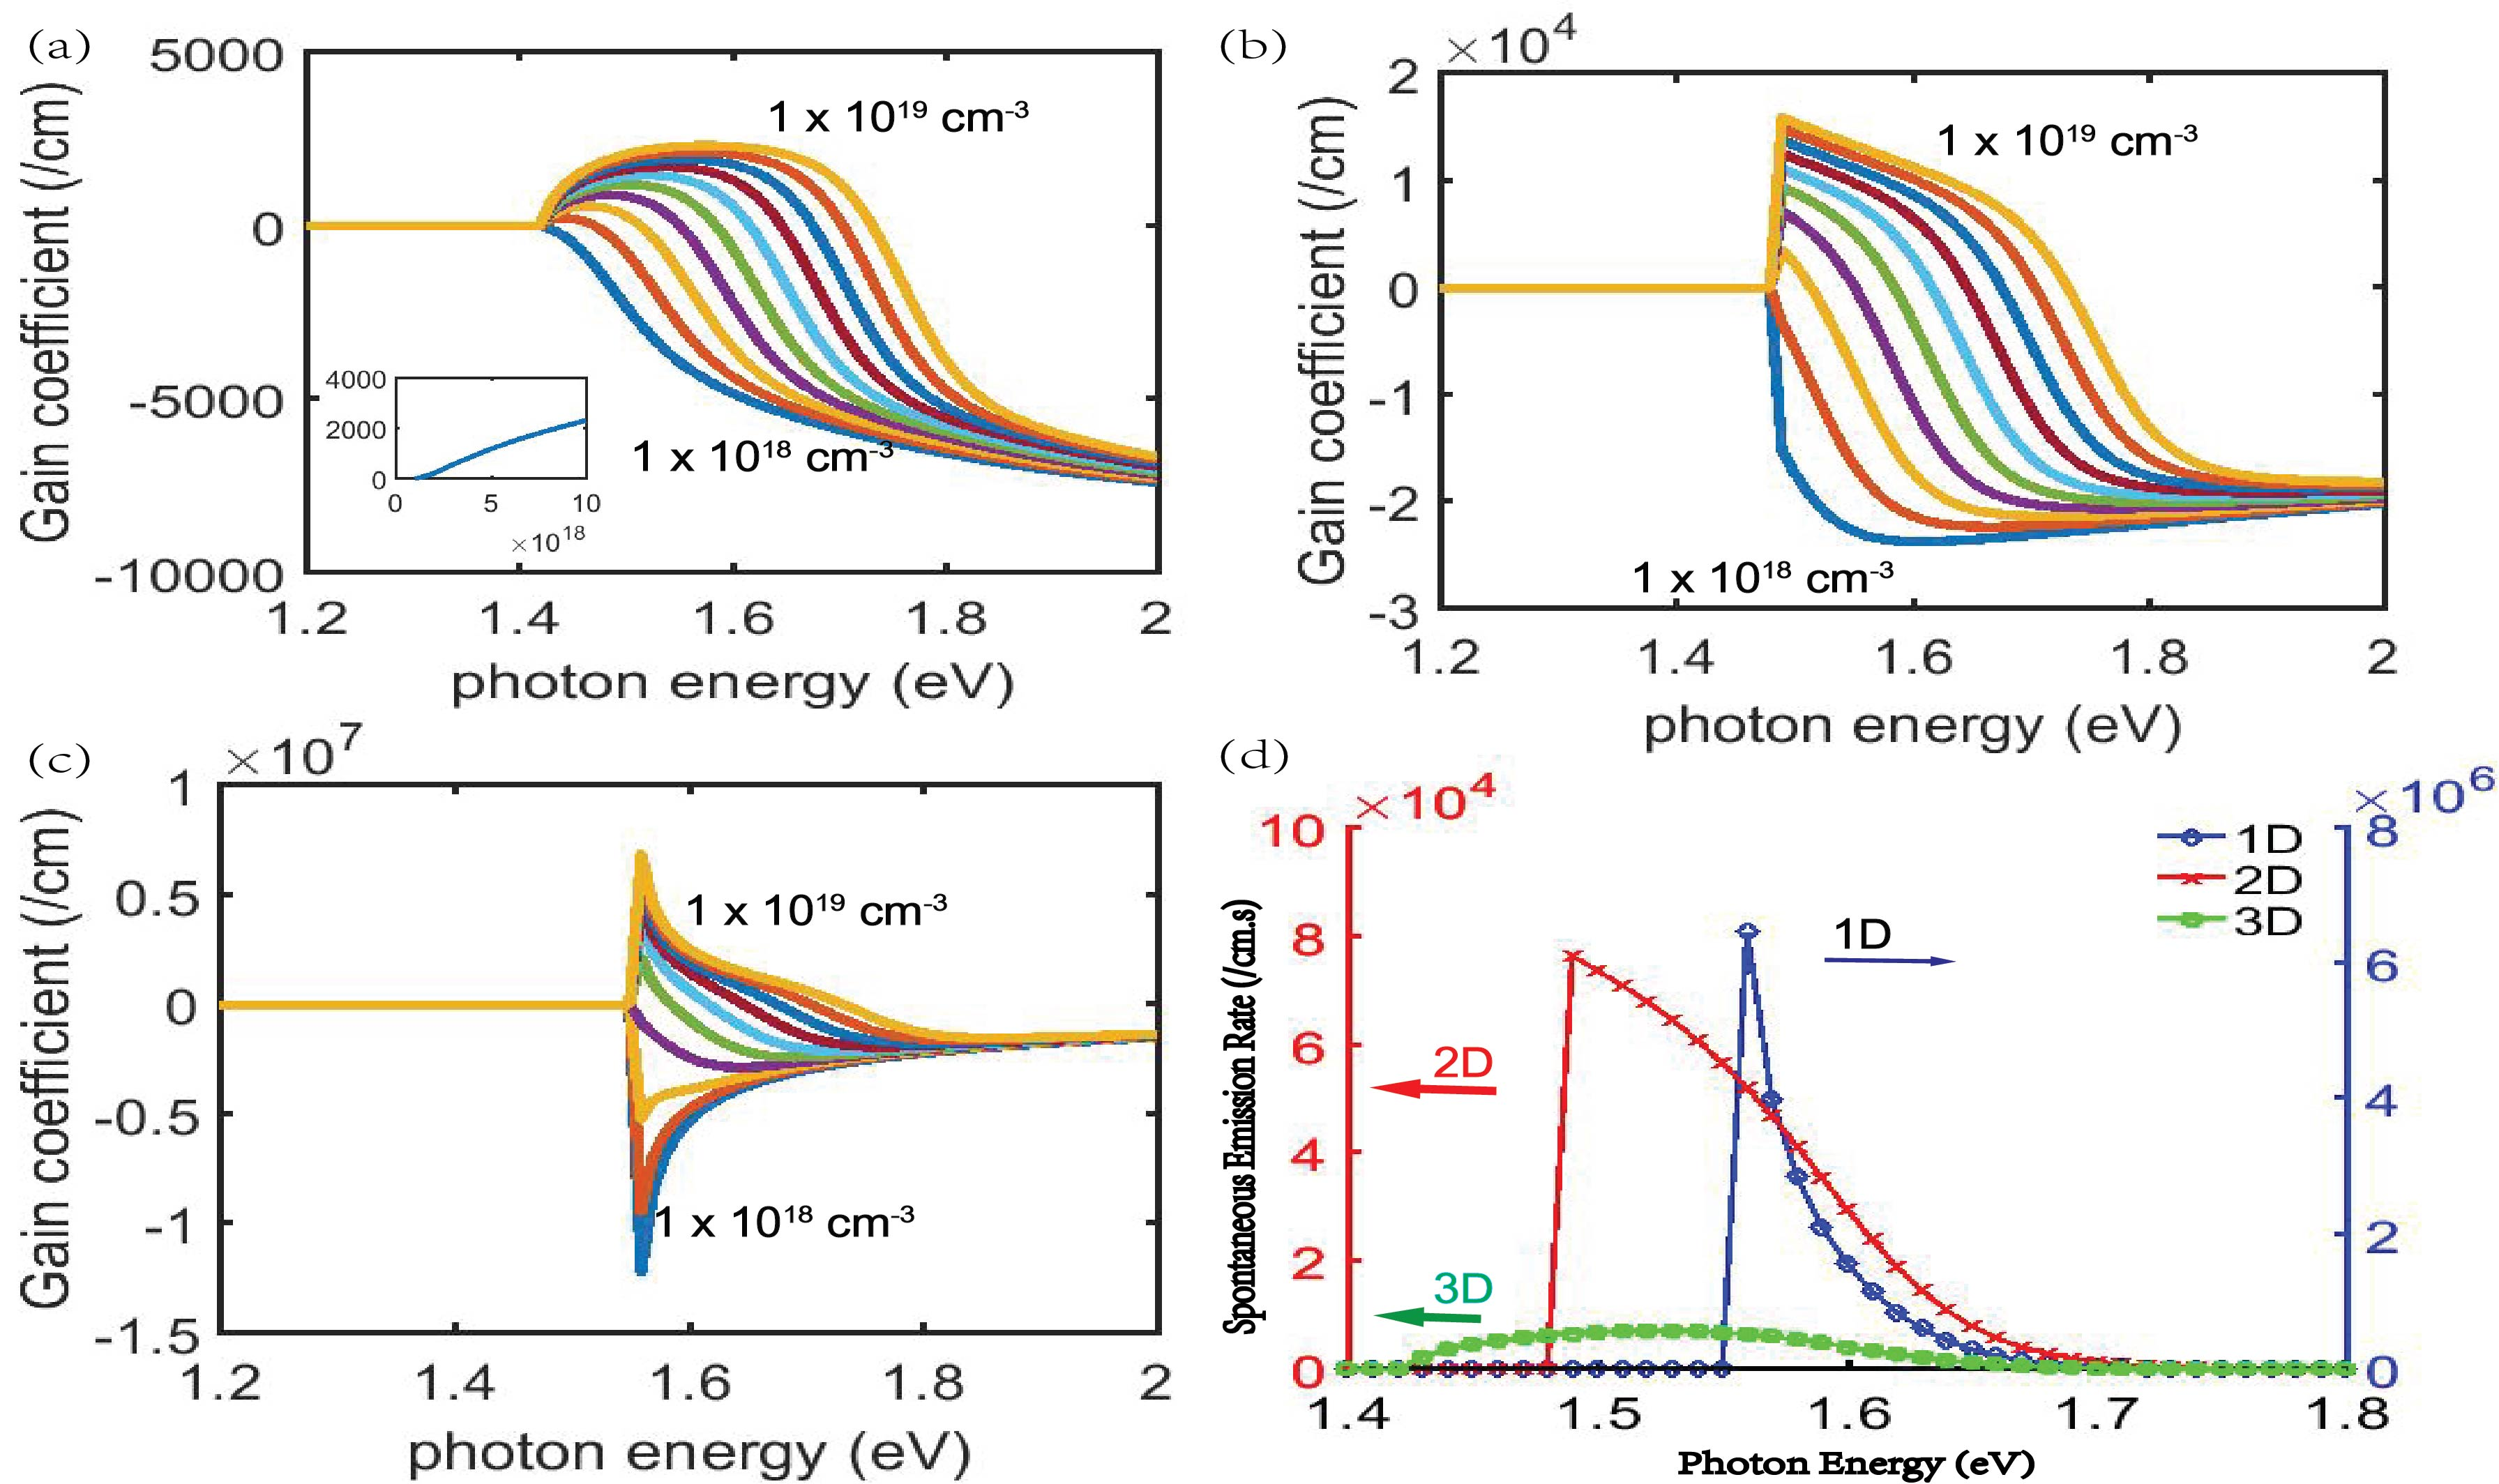
\includegraphics[width=\textwidth]{pictures/LT/gainspectrum}
  \label{gainspectrum}
\end{figure}

\begin{figure}
  \caption{Gain Model Fitting}
  \centering
  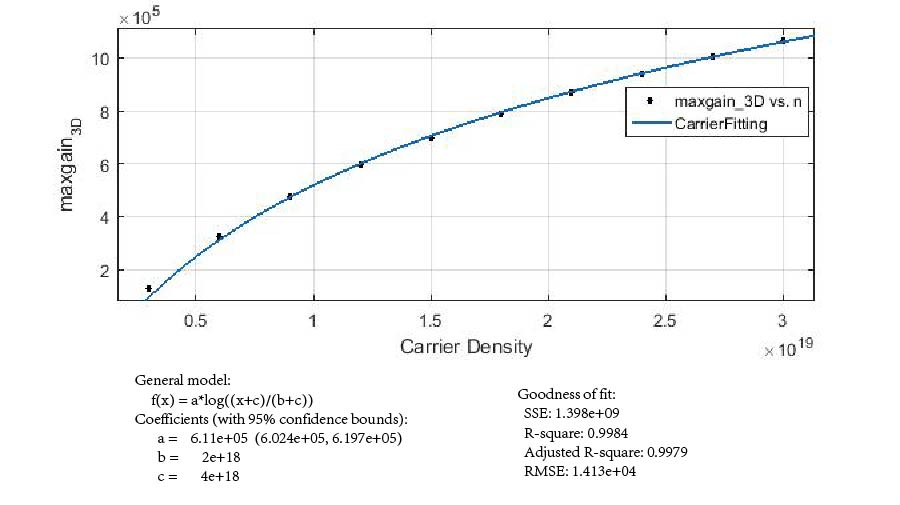
\includegraphics[width=\textwidth]{pictures/LT/gainModelFit_Anoted}
  \label{gainModelFit_Anoted}
\end{figure}

After fitting the curve in Fig.~\ref{gainModelFit_Anoted}, we can estimate the
threshold carrier density is $N_{th} = 4.533\times10^{18} cm^{-3}$. Then
plotting the spontaneous emission rate with respect to the threshold carrier
density $N_{th}$ for 3D, 2D and 1D as following:

\begin{eqnarray}
\begin{aligned}
& r_{3D}^{\mathrm{spon}}(\hbar\omega)=\frac{n_re^2\omega{p_{cv}^2}}{{\pi}\epsilon_0{m_0}^2C^3{\hbar}}\frac{{m_r^\ast}^{3/2}}{2\pi^2\hbar^3}{\sqrt{(\hbar\omega-E_g)}}f_n(\xi_2)(1-f_p(\xi_1)),
\\
& r_{2D}^{\mathrm{spon}}(\hbar\omega)=\frac{n_re^2\omega{p_{cv}^2}}{{\pi}\epsilon_0{m_0}^2C^3{\hbar}}\frac{{m_r^\ast}}{\pi\hbar^2L_z}f_n(\xi_2)(1-f_p(\xi_1)),
\\
& r_{1D}^{\mathrm{spon}}(\hbar\omega)=\frac{n_re^2\omega{p_{cv}^2}}{{\pi}\epsilon_0{m_0}^2C^3{\hbar}}\frac{{m_r^\ast}^{3/2}}{\pi\hbar{m_e^\ast}L_xL_y}\frac{1}{\sqrt{(\hbar\omega-E_g)}}f_n(\xi_2)(1-f_p(\xi_1)),
\end{aligned}
\label{eq:sponrates}
\end{eqnarray}

Figure~\ref{gainspectrum}(d) shows the spontaneous emission rate spectrum with
the estimated threshold carrier density for 3D(green), 2D(red) and 1D(blue)
based on Eqs.~\ref{eq:sponrates} with $(1+u_\varepsilon)\cong{1}$. Besides the
expected narrower linewidth, the peak rate for 1D is $6.4\times10^{6}
(cm^{-1})$, compared with $7.6\times10^{4} (cm^{-1})$ for 2D and
$7.1\times10^{3} (cm^{-1})$ for 3D.

The total spontaneous emission rate per unit volume per second is $R_{sp} =
\int_{\xi}r_{sp}d{\xi}$, and can be calculated for different dimensionalities
by integrating over entire photon energy spectrum, where $\xi=\hbar\omega$.
The optical output power created at threshold is $P_{out}=
h{\nu}{R_{sp}}|_{N_{th}}$.  The total generated optical output power at the
same injected carrier $N_{th}$ is seen to be 6.5 times and 175.3 times more for
2D and 1D, respectively, compared to the 3D case. In other words, with the same
amount of carriers injected either by optical pumping or electrical injection,
highly confined electronic structure can produce more than two orders of
magnitude more light compared to bulk.

%The threshold current for 3D is $2.62\times10^{27} (A/cm^2)$, 2D is
%$2.42\times10^{10} (A/cm^2)$, and 1D case is $4.73\times10^{6} (A/cm^2)$. The
%threshold current density needed for lower-dimensional structure is greatly
%reduced. Next, we can do dynamic analysis of laser modal and replace the threshold
%current density to threshold pumping power. And verify the result with the
%experimental data.

\section{Modeling of Nanowire Lasers} \label{SLModeling}

%FP semiconductor lasers produce a range of wavelengths. This range of
%wavelengths is called the "spectral width" of the laser. Typically there will
%be around 8 "modes" and the spectral width. In order to determin exactly the
%spectral shape, spectral width is usually quoted as the FWHM (Full Width Half
%Maximun) Instead of producing a continuous range of wavelengths over their
%spectral width. Semiconductor lasers produce a series of "lines" at a number
%of discrete wavelengths. Lines themselves vary in width (in different types of
%lasers) very significantly. The linewidth is inversely proportional to the
%coherence length of the laser.
%
In this section, we model an idealized semiconductor nanowire laser from the
general formulations through the rate equations and wave equations based on the
generalized Fabry-Perot (FP) lasers.

Considering different aspects of the energy conservation rule, there are two
basic classical methods to model the operation of semiconductor lasers. The
first method applies the concept of photon/electron particles exchange with the
abstract optical parameters and is suitable for the FP lasers as depicted in
Fig.~\ref{FPLasingMechanism}. The FP laser is conceptually a cavity with a pair
of end mirrors or facets. The mirrors are needed to create the feedback
mechanism of light inside an amplifying medium for lasing to occur. The lasing
medium can only amplify (undergo stimulated emission) over a fairly narrow
range because of the characteristics of the material. On the other hand, strong
non-uniformities of index distribution of the DBR/DFB lasers alters the
interaction between electromagnetic fields and the electronic particles. These
two methods are compatible with each another. Here, because the nanowire based
lasers have net propagating resonant mode in the axial direction and the
resonant modes are very similar to the FP modes, we employ the first method,
which is the standard rate equation approach.

\begin{figure}
  \caption{Schematic diagram of a semiconductor Fabry-Perot laser}
  \centering
  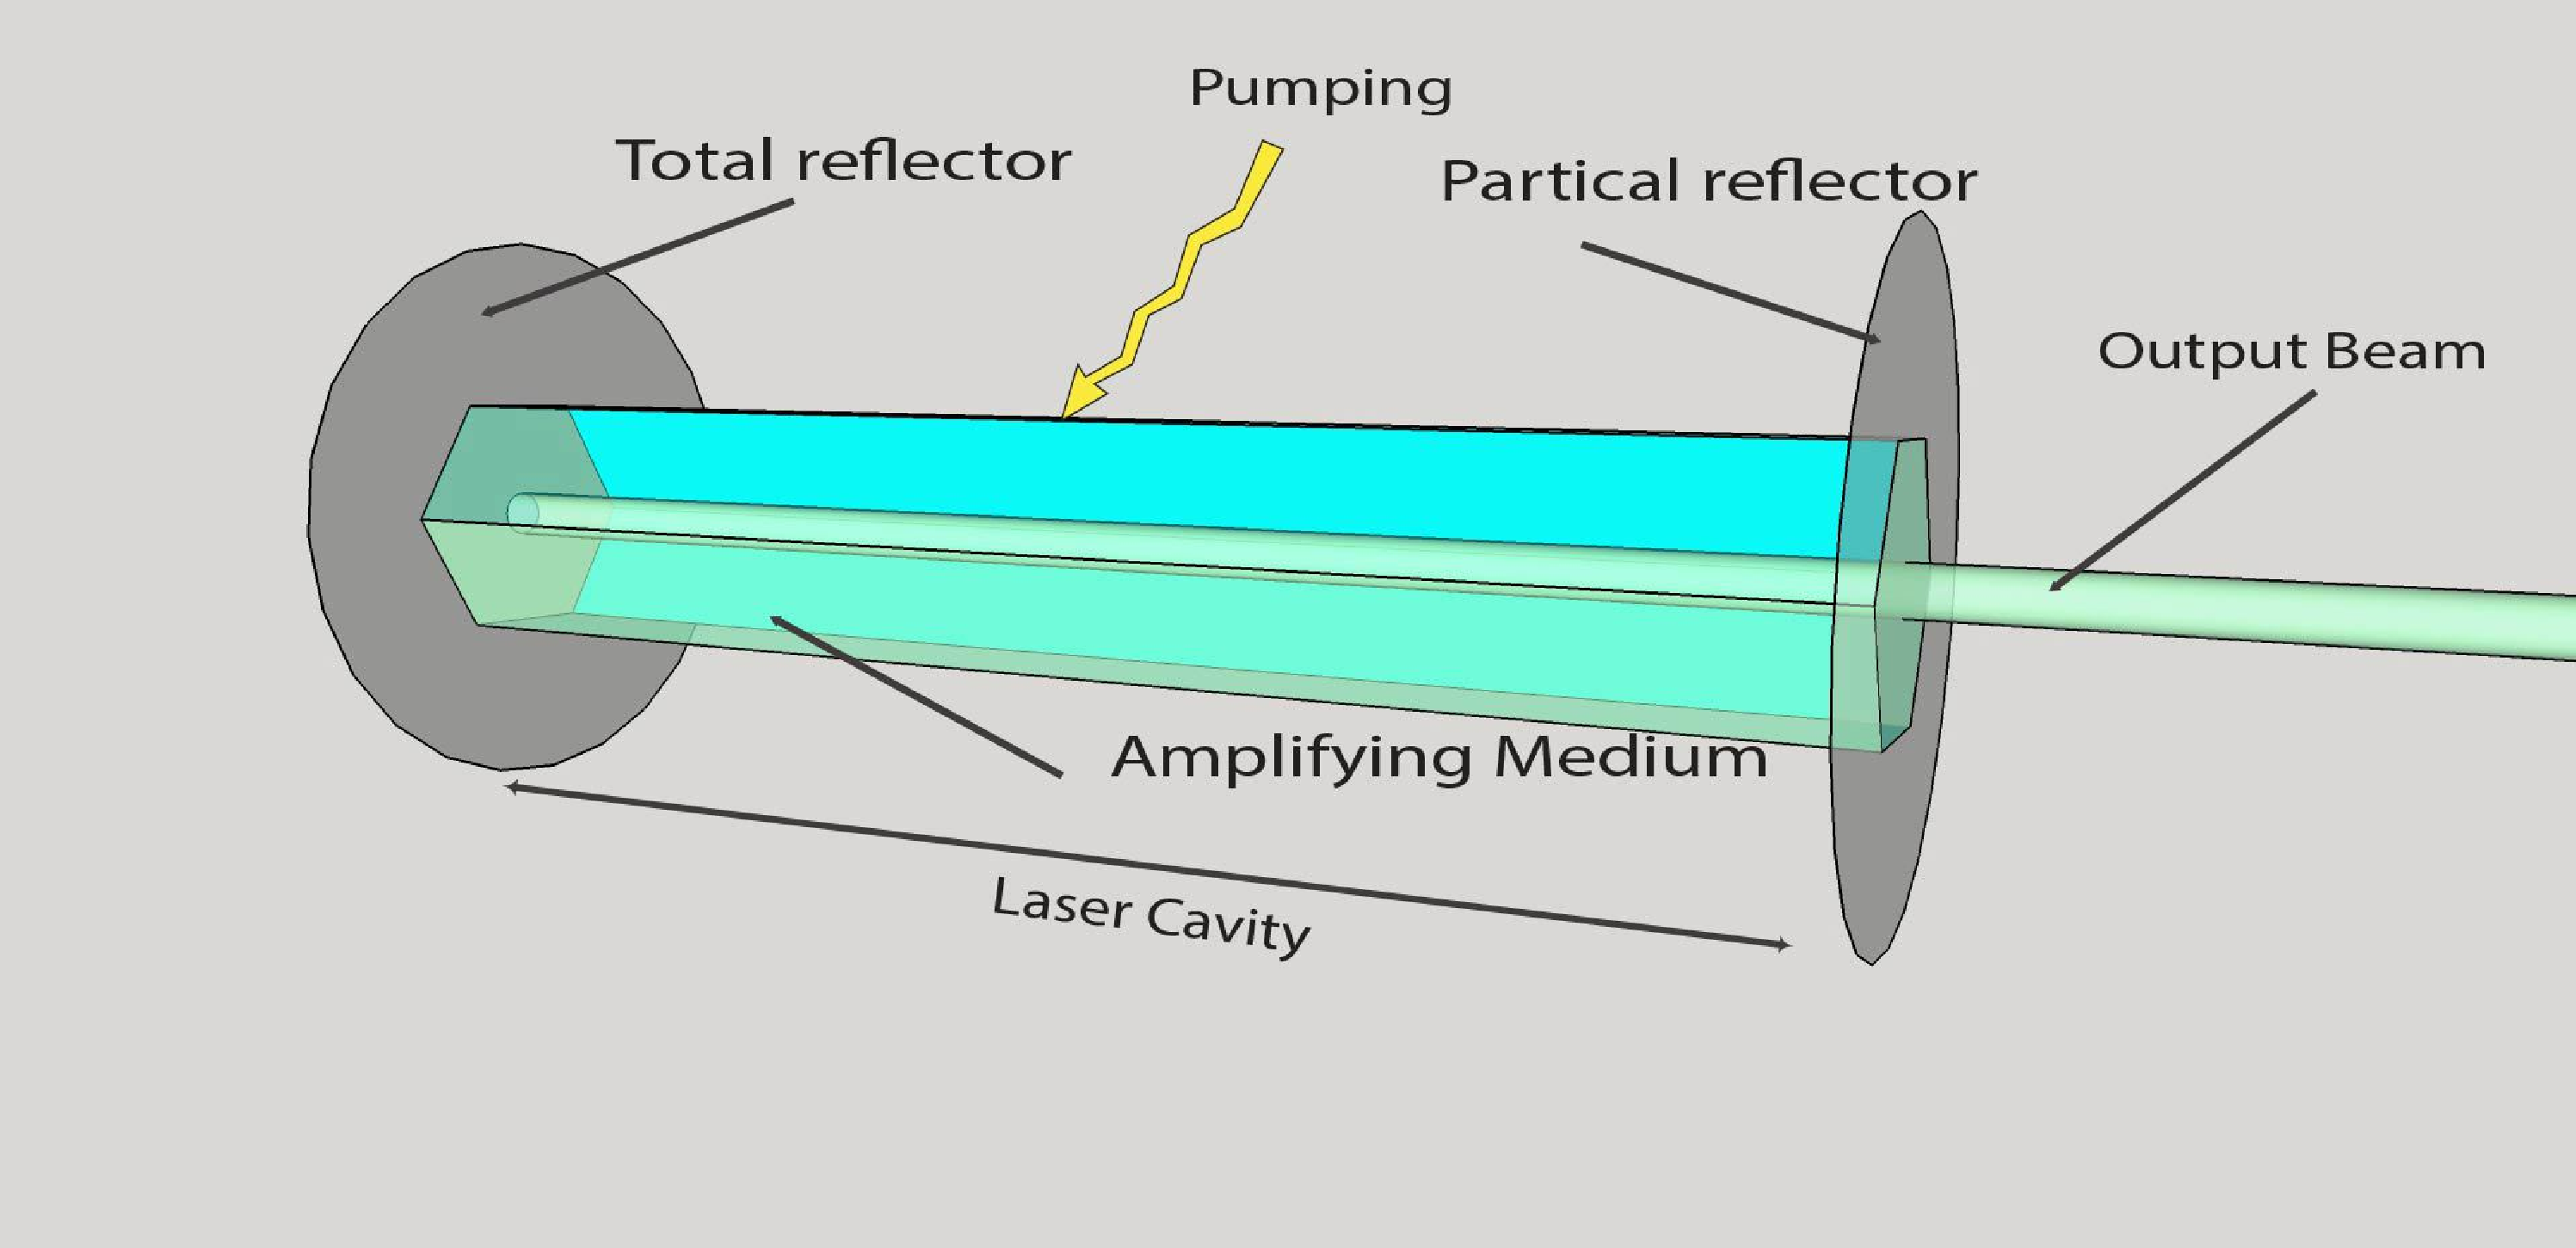
\includegraphics[width=\textwidth]{pictures/LT/FPLasingMechanism}
  \label{FPLasingMechanism}
\end{figure}

As discussed previously, there are three fundamental elements in the
semiconductor lasers: semiconductor band structure, current injection/optical
pumping, and cavity. The former two are related to the material and junction
structure, and the later is related to the laser structure. The key part of
modeling semiconductor laser is to deal with the interaction between
electromagnetic fields and gain medium. Figure~\ref{NWLaserModeling}
illustrated the basic procedure of modeling semiconductor nanowire lasers.
Starting from the optical pumping power, the carrier density, $N$, can be
calculated by solving Poisson and carrier continuity equations. Then some
optical parameters, such as effective refractive index and confinement factor
related to the optical modes, can be extrapolated from the FDTD simulation
results. Simultaneously, the optical gain of the gain medium is given by the
optical transition rate equations. Finally, the optical output power is
proportional to the photon density $N_p$, which is numerically solved by the
rate equations and coupling between carrier and photon density using the
traveling-wave approach (in time domain).  It solves the time-dependent
coupled-wave equations for the forward and the backward traveling waves
directly and therefore is valid even the laser cavity has relatively small
Q-factor and/or the characteristic time of the laser dynamics is very short.
Of importance, the traveling-wave model can be applied to lasers operated with
multiple cavity modes which is the case for the as-grown core-shell nanowires.

\begin{figure}
  \caption{Flow chart diagram of modeling a semiconductor nanowire laser.}
  \centering
  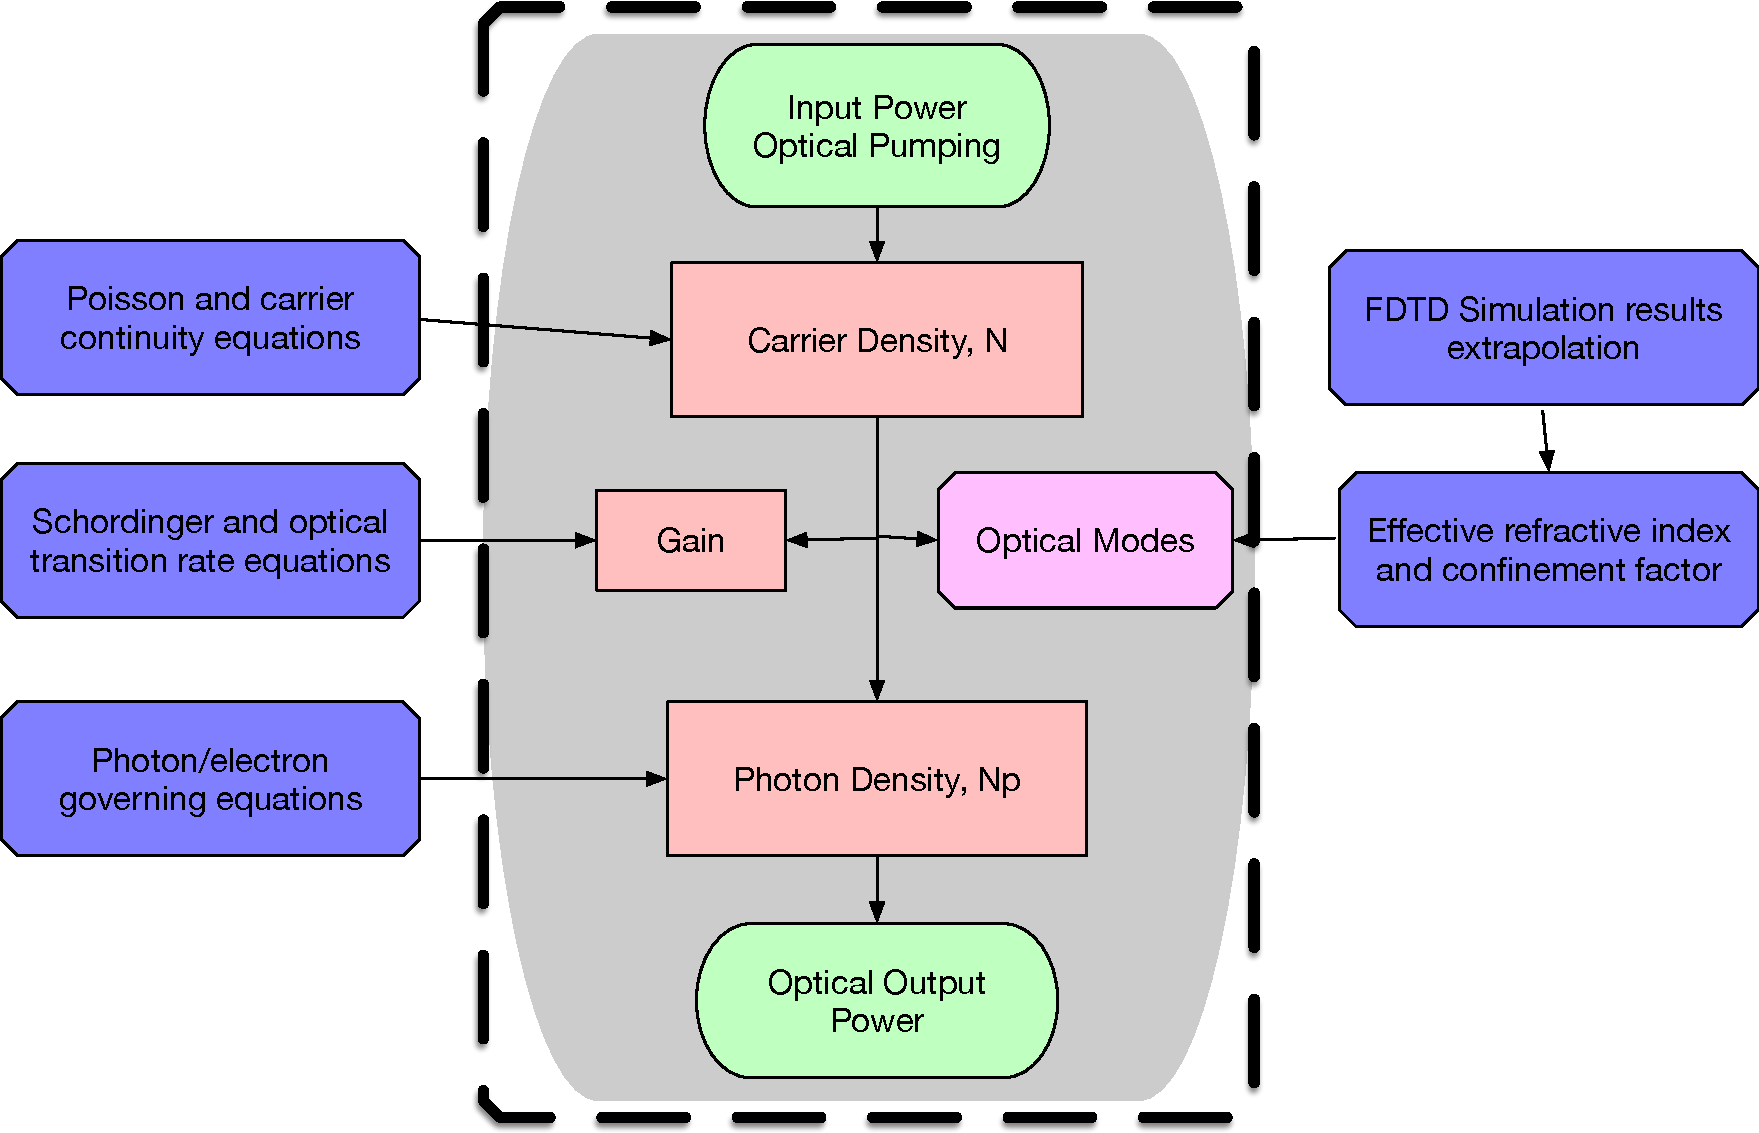
\includegraphics[width=\textwidth]{pictures/LT/NWLaserModeling}
  \label{NWLaserModeling}
\end{figure}

\section{Laser Rate Equations} \label{LaserRateEq}

We start with the governing equations of carrier density $N$ and photon density
$N_p$ in the active region of a semiconductor laser which is governed by a
dynamic process~\cite{coldren2012diode}:

\begin{eqnarray}
\begin{aligned}
  & \frac{dN}{dt} = \frac{\eta_{i}I}{qV} - \frac{N}{\tau} - R_{st},
  \\
  & \frac{dN_p}{dt} = {\Gamma}v_g{g}N_p + \Gamma\beta_{sp}R_{sp} - \frac{N_p}{\tau_p},
\end{aligned}
\label{eq:governingI}
\end{eqnarray}

where $\beta_{sp}$ is the spontaneous emission factor, defined as the
percentage of the total spontaneous emission coupled into the lasing mode. And
it is just the reciprocal of the number of available optical modes in the
bandwidth of the spontaneous emission for uniform coupling to all modes. The
$g$ is the incremental gain per unit length. $\eta_i$ is the injection
efficiency, which defined as the fraction of terminal current that generates
carriers in the active region. $\tau$ and $\tau_p$ is the carrier lifetime and
photon lifetime, respectively.

The first term on the right hand side of equation~\ref{eq:governingI}(top) is
the generation rate of injected electrons $G_{gen} = {\Gamma_{i}I}/{qV}$, where
${\Gamma_{i}I}/{q}$ is the number of electrons per second being injected into
the active region, where V is the volume of the active region. The rest terms
are the rate of recombining of electrons per unit volume in the active region.
There are several mechanisms should be considered, including a spontaneous
recombination rate, $R_{sp}$, a nonradiative recombination rate, $R_{nr}$, a
carrier leakage rate, $R_l$ and a net stimulated recombination, $R_{st}$,
including both stimulated absorption and emission. Thus, the total
recombination rate is the sum of all rates:

\begin{equation}
  R_{rec} = R_{sp} + R_{nr} + R_{l} + R_{st}
  \label{eq:recrate}
\end{equation}

The first three terms on the right refer to the natural or unstimulated carrier
decay processes. The fourth one, $R_{st}$, require the presence of photon.

Equation~\ref{eq:governingI} uses input current intensity, $I$, for
electrically injected lasing situation, however, if optical pump, $P$, used as
the lasing source, then we need to rewrite the governing equations as:

\begin{eqnarray}
\begin{aligned}
  & \frac{dN}{dt} = \frac{\eta_{i}P}{h\nu{V}} - \frac{N}{\tau} - R_{st},
  \\
  & \frac{dN_p}{dt} = {\Gamma}v_g{g}N_p + \Gamma\beta_{sp}R_{sp} - \frac{N_p}{\tau_p},
\end{aligned}
\label{eq:governingP}
\end{eqnarray}

$P$ is the optical pump used for exciting nano-cavity laser emission and is
time-dependent of the form $P_{p}sech^2(\frac{1.76t}{\delta{t}})$, where $P_p$
is the peak power amplitude, and $\delta{t}$ is the time pulse width.

The cavity loss can be characterized by a photon decay constant or lifetime,
$\tau_p$, and the threshold can be reached when the round trip gain overcomes
losses.  By assuming steady-state conditions (\ie $dN_p/dt = 0$), and solving
for this steady-state or threshold gain, $g_{th}$, where the generation term
equals the recombination term for photons. We assume only a small fraction of
the spontaneous emission is coupled into the mode (\ie $\beta_{sp}$ is quite
small), and only consider light emission into a single mode of the resonant
cavity, then the second term can be neglected, and we have the solution:

\begin{equation}
  \Gamma{g_{th}} = \frac{1}{v_g\tau_p} = <\alpha_i> + \alpha_m
\end{equation}

The product, $\Gamma{g_{th}}$, is referred to as the threshold modal gain
because it represents the net gain required for the mode as a whole that
experiences the cavity loss. $<\alpha_i>$ is the average internal loss, and
$\alpha_m$ is the mirror loss if we considered an in-plane wave laser. However,
since the refractive index difference between CSNW and the Si or GaAs substrate
is very small, we may change the mirror loss into leaky loss due to the
confined volumetric resonant mode $\alpha_l$.

At threshold, the steady-state carrier rate equation can be expressed as:

\begin{equation}
  \frac{\eta_{i}P_{th}}{h\nu{V}} = {(R_{sp} + R_{nr} + R_{l})}_{th}=\frac{N_{th}}{\tau}
  \label{eq:steadyrate}
\end{equation}

where $(R_{sp} + R_{nr} + R_{l}) =AN + BN^2 +CN^3$ depends monotonically on
$N$, and this recombination rate will saturate at its threshold value.  Thus,
we can substitute Eq~\ref{eq:steadyrate} into the carrier rate equation
Eq~\ref{eq:governingP} to obtain an above threshold carrier rate equations:

\begin{equation}
  \frac{dN}{dt} = \eta_i \frac{(P - P_{th})}{h\nu{V}} - v_{g}gN_p,~~~   (P > P_{th})
\end{equation}

The steady-state photon density can be also calculated when pumping power above
threshold where $g = g_{th}$,

\begin{equation}
  N_p = \frac{\eta_i (P - P_{th})}{h{\nu}v_{g}g_{th}V}~~~   (steady~ state)
\end{equation}

Then the optical output power intensity is obtained
by multiplying the photon density, $N_p$, by the energy per
photon, $hv$, and the group velocity, $g_v$.

\begin{equation}
  P_{op} = \frac{\eta_{i}(P-P_{th})}{g_{th}V}
\end{equation}

Therefore, the optical output power is simply calculated as:

\begin{equation}
  P_0 = P_{op}wd =\eta_i\frac{(P-P_{th})wd}{g_{th}V}=\eta_i\frac{(P-P_{th})}{g_{th}L}~~~(P > P_{th})
\end{equation}

where $w$, $d$ and $L$ are the width, thickness and length of the active
region, respectively. All input parameters for the modeling of semiconductor
nanowire laser are listed in Table~\ref{tab:Inputpara_SL}.

\setlength{\tabcolsep}{4pt}

\begin{deluxetable}{lll}
\tabletypesize{\footnotesize}
\tablewidth{0pt}

\tablecaption{Input parameters of the core-shell nanowire semiconductor laser. \label{tab:Inputpara_SL}}
\tablehead{\colhead{Parameters} & \colhead{Symbol} & \colhead{Values and Units}}
\startdata
Cavity length                           &   {\em L}            &  $3\quad {\mu}m$\\
Active-region width                     &   {\em w}            &  $300\quad nm$\\
Active-region thickness                 &   {\em d}            &  $300\quad nm$\\
Carrier lifetime                        &   {\em $\tau_{r}$}   &  1\quad ns\\
Spontaneous emission lifetime           &   {\em $\tau_{sp}$}  &  1\quad ns\\
Gain coefficient                        &   {\em $g_0$}        &  $3.0\times10^{-16}\quad cm^{-2}$\\
Carrier density at threshold            &   {\em $n_{th}$}     &  $4.5\times10^{18}\quad cm^{-3}$\\
Cavity loss                             &   {\em $\alpha_{c}$} &  $20\quad cm^{-1}$\\
Pumping power                           &   {\em $p_{0}$}      &  $200\quad \mu{W}$\\
Reference wavelength                    &   {\em $\lambda_{0}$}&  $800\quad nm$\\
Planck's constant                       &   {\em h}            &  $6.625\times10^{-34}\quad Js$\\
Electron charge                         &   {\em e}            &  $1.6\times10^{-19}\quad C$\\
Nonradiative recombination coefficient  &   {\em A}            &  $1.43\times10^{8}\quad s^{-1}$\\
Auger recombination coefficient         &   {\em C}            &  $3.5\times10^{-30}\quad cm^{6}\cdot{s}$\\
\enddata
\tablecomments{The rest of the parameters that are not listed here have its conventional meaning and values.}
\end{deluxetable}


It is desirable to reduce the cavity loss $(<\alpha_i> + \alpha_m)$ and volume,
$V$, in order to retaining a reasonably large confinement factor, $\Gamma$.
However, CSNWs based semiconductor laser as a good resonant cavity are able to
confine light with a large quality factor. The extrapolated confinement
factor based on the FDTD simulation results is 0.756, along with other
calculated parameters listed in Table~\ref{tab:Calcpara_SL}.

\setlength{\tabcolsep}{4pt}

\begin{deluxetable}{llll}
\tabletypesize{\footnotesize}
\tablewidth{0pt}

\tablecaption{Calculated parameters of core-shell nanowire semiconductor laser. Some of the parameters are calculated based on the FDTD simulation results. \label{tab:Calcpara_SL}}
\tablehead{\colhead{Parameters} & \colhead{Symbol} & \colhead{Values and Units} & \colhead{Reference}}
\startdata
Area of top section of active part      &   {\em $A_I$}       &  $9.0\times10^{5}~nm^{2}$ &  $A_I=Lw$    \\
Area of cross section of active part    &   {\em $A_{p}$}     &  $9.0\times10^{4}~nm^{2}$ &   $A_p=wd$ \\
Effective refractive index              &   {\em $n_r$}       &  $2.728$  &\\
Group refractive index                  &   {\em $n_{g}$}     &  $3.5$    &\\
Group velocity of light                 &   {\em $v_{g}$}     &  $8.56\times10^{7}~m/s$ $v_g=c/{n_g}$  \\
Confinement factor                      &   {\em $\Gamma$}    &  0.756   \\
Photon lifetime                         &   {\em $\tau_{ph}$} &  5.84 ps   &  $\tau_{ph}=I/v_g\alpha_c$  \\
Gain coefficient for power              &   {\em $g_p$}       &  $1.94\times10^{-12}~ cm^3/s$   & $g_p=\Gamma{v_g}g_0$  \\
Pumping power density                   &   {\em $P_0$}    &  $2.22\times10^9~W/m^2$   & $P_0=p_0/A_p$  \\
Carrier density at transparency         &   {\em $n_0$}       & $4.41\times10^{18}~ cm^{-3}$    \\
Threshold pumping power density         &   {\em $P_{th}$}    &  $3.35\times10^8~W/m^2$   \\
The operating frequency                 &   {\em $f$}         &  $3.75\times10^{14}~Hz$   &  $f=c/\lambda_0$ \\
Threshold pumping power                 &   {\em $Power_{th}$}      &  $3.0\times10^{-5}~W$   &  $Power_{th}=P_{th}A_p$ \\
Analytical power                        &   {\em $P_{analyt}$}       &  $0.439~W$   \\
\enddata
\tablecomments{The rest of the parameters that are not listed here have its conventional meaning and values.}
\end{deluxetable}


Now, we are able to generate the transient responses of carrier and photon
densities with respect to the pumping power. Figure~\ref{L-L} shows the optical
output power versus the input pumping power with a threshold pumping power at
$30 \mu{W}$. The gain switching occurs because of ultrafast excitation. By
generating a large amount of carriers at a very short times cale, picosecond
pump pulses excite carrier densities significantly above threshold, resulting
in a strong peak of stimulated emission as shown in Fig.~\ref{SteadyPower} and
Fig.~\ref{SteadyGain}. Thus, the optical output power reaches maximum value
when the gain at its maxim, and quickly drops below threshold after this
initial spike.

\begin{figure}
  \caption{Calculated optical output power vs. pumping power, i.e., L-L curve.}
  \centering
  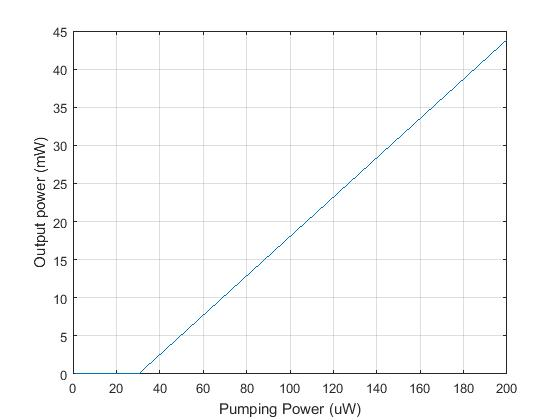
\includegraphics[width=0.8\textwidth]{pictures/LT/L-L}
  \label{L-L}
\end{figure}

\begin{figure}
  \caption{The calculated steady state optical output power.}
  \centering
  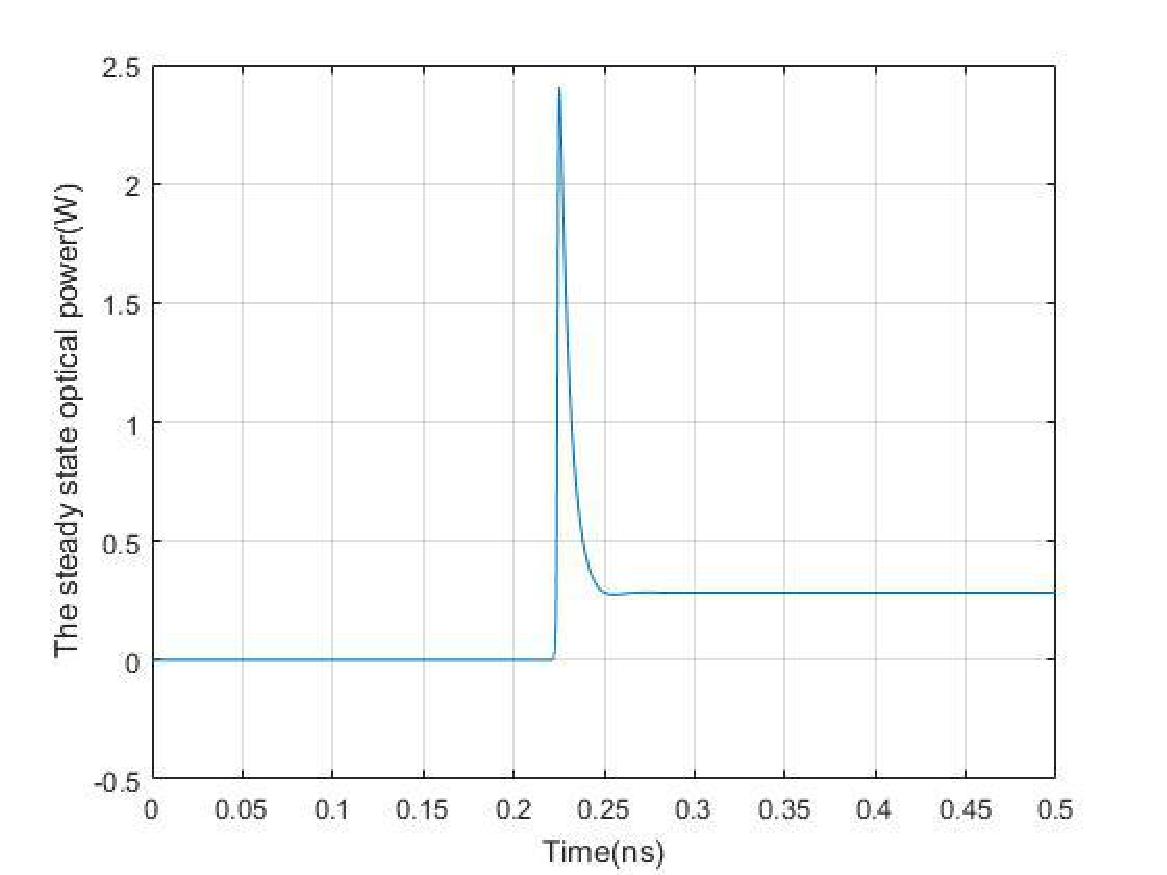
\includegraphics[width=0.8\textwidth]{pictures/LT/SteadyPower}
  \label{SteadyPower}
\end{figure}

\begin{figure}
  \caption{The calculated steady state gain $G_m$ of semiconductor nanowire laser.}
  \centering
  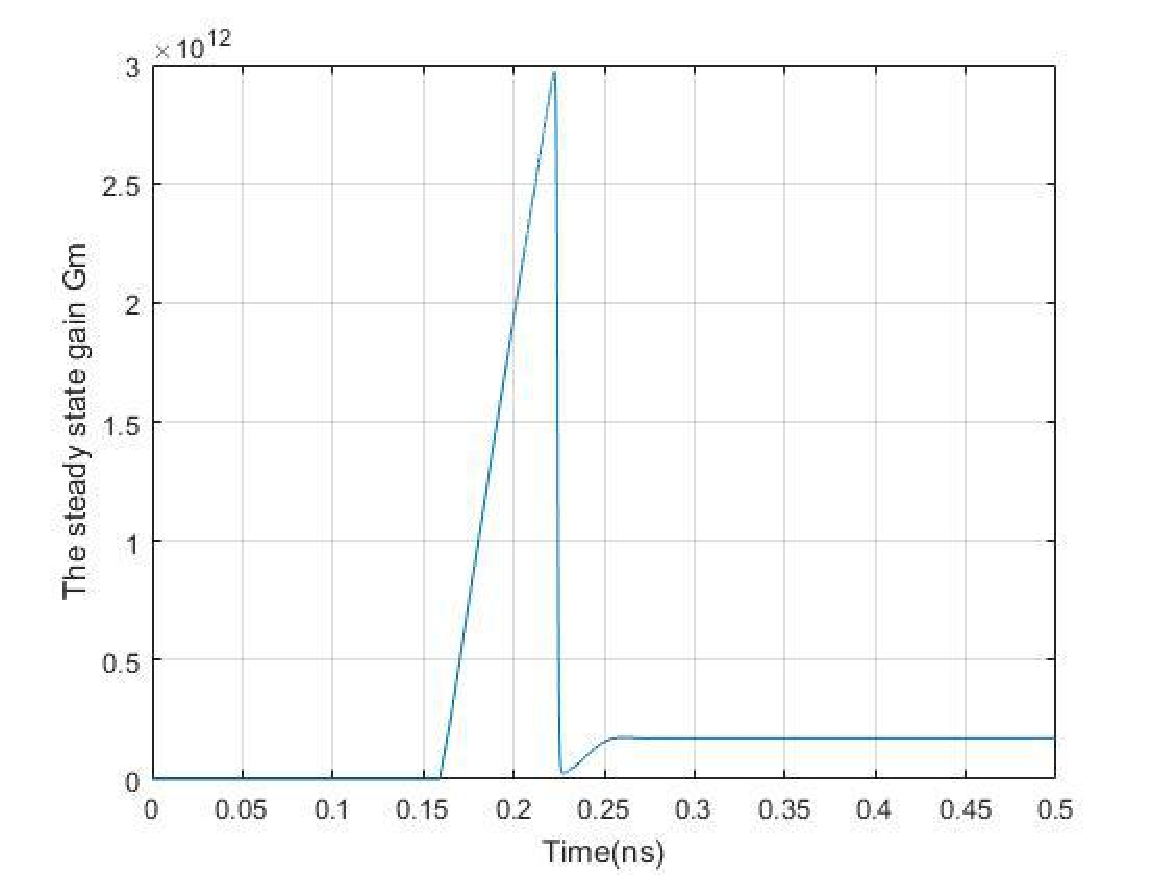
\includegraphics[width=0.8\textwidth]{pictures/LT/SteadyGain}
  \label{SteadyGain}
\end{figure}

\section{Linewidth Enhancement Factor} \label{Linewidth}

Electrons and holes frequently interact with other carriers and with phonons,
thereby changing their energy within the sub-band. Such intra-band scatter
events happen about every 0.1 ps, much more often than band-to-band
recombination events. Thus, scattering leads to an uncertainty of the electron
energy, which can be accounted for by introducing a symmetrical linewidth
broadening function $L$ into the gain formula~\cite{Piprek:2013wu}.  In fact,
positive gain is now possible even for photon energies slightly below the
bandgap. Cauchy himself exploited such a density function in
1827~\cite{stigler2002statistics}, with an infinitesimal scale parameter, in
defining a Dirac delta function, while among physicists, it is known as the
Lorentzian lineshape function $L$ as in Eq.~\ref{eq:LorentzianEq} with the
half-width. This function is based on the assumption that the occupation
probability of an electron state decays proportionally to
${exp}^{(-{t}/{\tau})}$. And the Fourier transformation of this exponential
function into the energy domain gives the Lorentzian lineshape function.

\begin{equation}
L(E-E_{21})=\frac{1}{\pi}\frac{\hbar/\tau_{in}}{{(\hbar/\tau_{in})}^2+{(E-E_{21})}^2}
\label{eq:LorentzianEq}
\end{equation}

The intraband relaxation time, $\tau_{in}$, is the tiem constant associated
with the exponetial decay of the elctron. $\Gamma=\hbar/\tau_{in}$ is the
average of the broadening in the conduction and in the valence band. The full
linewidth $2\Gamma$ is related to the average intra-band scattering time, which
includes scattering events in the conduction band and valence band. For each
band, linewidth contributions from different scattering processes are adding
up. This convolution integral means that gain at the photon energy can now
receive contributions from electron transitions within sub-bands.
